\documentclass[12pt,a4paper]{report}

\usepackage[utf8]{inputenc}
\usepackage[T1]{fontenc}
\usepackage{mathpazo}
\usepackage[english]{babel}
\usepackage{amsmath}
\usepackage{amsfonts}
\usepackage{amssymb}
\usepackage{wrapfig}
%\usepackage{times}
\usepackage{graphicx}
\usepackage{listings}
\usepackage{float}
\usepackage[backref, hidelinks, urlcolor=blue]{hyperref}
\usepackage[nottoc]{tocbibind}

\oddsidemargin -0.25in		% Left margin is 1in + this value
\textwidth 6.75in		% Right margin is not set explicitly
\topmargin 0in			% Top margin is 1in + this value
\textheight 9in			% Bottom margin is not set explicitly
\columnsep 0.25in		% separation between columns

\author{Adrian-Gabriel Bălănescu}
\title{Reinforcement learning lab report}
\begin{document}
	\maketitle
	\tableofcontents
	
	\chapter{Game description}
		\emph{Gravitar} is an arcade style game released by Atari in 1982. The game was known for its high level of difficulty \cite{noauthor_gravitar_2021}.
		
		\begin{wrapfigure}{r}{0.28\textwidth}
			\begin{center}
				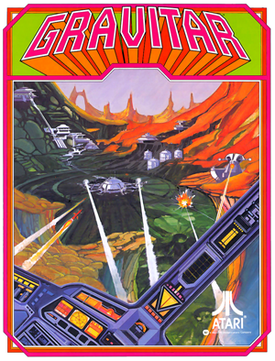
\includegraphics[width=0.32\textwidth]{Gravitar.png}
			\end{center}
			\caption{Gravitar logo}
		\end{wrapfigure}
		
		\section{Gameplay}
	
		The game takes place in a fictional solar system. The player controls a spacecraft with the help of five buttons: two to rotate the ship left and right, one to shoot, one to activate the thruster and one for both a tractor beam and a force field. In the side-view levels, the player has to destroy red bunkers that shoot constantly, and can also use the tractor beam to pick up blue fuel tanks. Once all of the bunkers are destroyed, the planet will blow up, and the player will earn a bonus. Once all planets are destroyed, the player will move onto another solar system.
		The player will lose a life if he crashes into the terrain or gets hit by an enemy's shot, and the game will end immediately if fuel runs out \cite{noauthor_gravitar_2021}.
		
		
		After completing all 11 planets (or alternatively completing the reactor three times) the player enters the second universe and the gravity will reverse. Instead of dragging the ship towards the planet surface, the gravity pushes it away. In the third universe the landscape becomes invisible and the gravity is positive again. The final, fourth universe, has invisible landscape and reverse gravity. After completing the fourth universe the game starts over
		 \cite{noauthor_gravitar_2021}.
		 
		 \pagebreak
		 
		\begin{figure}[ht!]
			\begin{minipage}[c]{0.5\linewidth}
				\centering
				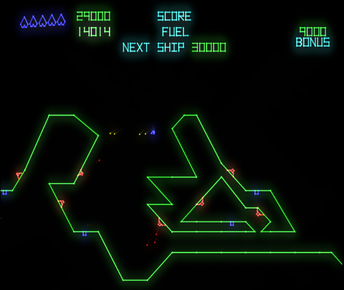
\includegraphics[height=0.3\textheight, width=0.9\linewidth]{Gravitar2.png}
				\caption{A level from Gravitar}
			\end{minipage}\hfill
			\begin{minipage}[c]{0.5\linewidth}	
				\centering
				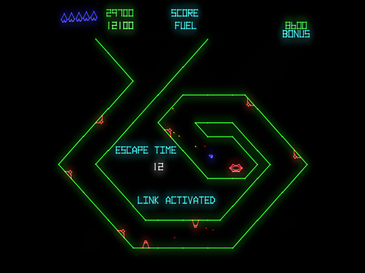
\includegraphics[height=0.3\textheight, width=0.9\linewidth]{Reactor.png}
				\caption{The reactor}
			\end{minipage}
		\end{figure}
	
		\section{Gravitar in SLM-lab}
		
		\emph{SLM-lab} \cite{kenggraesser2017slmlab} is a software framework for reproducible reinforcement learning (RL) research. It implements most of the canonical RL algorithms in a modular platform that allows for easy experimentation and analysis. It includes the OpenAI Gym \cite{brockman2016openai} environments, which contains a lot of Atari games emulations, one being Gravitar.
		
		In this environment, the observation is an RGB image of the screen, which is an array of shape \lstinline|(210, 160, 3)|. Each action is repeatedly performed for a duration of $k$ frames, where $k$ is uniformly sampled from $\{2, 3, 4\}$. The action space is discrete and has 18 available commands like fire, up, down, right, left and so on.
		
		The Gravitar environment can be loaded in SLM-lab by specifying in the \lstinline|.json| configuration file, at the \lstinline|"env"| section the \lstinline|"name"| of the environment. In this case, \lstinline|"GravitarNoFrameskip-v4"|. 
		
	\chapter{Algorithms}
		In this chapter, the algorithms used will be briefly explained.
		\section{DQN - Deep Q-Network}
		...
		\section{A2C - Advantage Actor-Critic}
		...
		\section{PPO - Proximal Policy Optimization}
		...
		\section{SAC - Soft Actor-Critic}
		...
	\chapter{Experimental Results}
	(here please provide, for each algorithm, the full config file, the description of the config, similar to those in the course, and the graphs of the results; try to train each algorithm for at least 500k-1M steps; make sure to train all the algorithms for the same number of steps)
	\chapter{Conclusions}
	(here please discuss the results obtained and compare the performance of the algorithms)
	
	\bibliographystyle{unsrt}	% Order by citation
	\bibliography{lab_report_bibliography.bib}
	
\end{document}